% Created 2016-05-31 Tue 19:33
% Intended LaTeX compiler: pdflatex
\documentclass[bigger]{beamer}
\usepackage[utf8]{inputenc}
\usepackage[T1]{fontenc}
\usepackage{graphicx}
\usepackage{grffile}
\usepackage{longtable}
\usepackage{wrapfig}
\usepackage{rotating}
\usepackage[normalem]{ulem}
\usepackage{amsmath}
\usepackage{textcomp}
\usepackage{amssymb}
\usepackage{capt-of}
\usepackage{hyperref}
\usepackage{listings}
\usepackage{float}
\usepackage{fontspec}
\setsansfont{Arial}
\usepackage[english, greek]{babel}
\usepackage[iso-8859-7]{inputenc}
\usetheme{default}
\author{Χρήστος Περιβολαρόπουλος}
\date{Τετάρτη 8 Ιουνίου 2016}
\title{Εξαγωγή σχεσιακών πληροφοριών από τη Βικιπαίδια}
\hypersetup{
  pdfauthor={Χρήστος Περιβολαρόπουλος},
  pdftitle={Εξαγωγή σχεσιακών πληροφοριών από τη Βικιπαίδια},
  pdfkeywords={},
  pdfsubject={Making sense of semi structured data in wikipedia.},
  pdfcreator={Emacs 24.5.1 (Org mode 8.3.3)},
  pdflang={English}}

\newenvironment{code}{\ttfamily}{\par}

\newcommand{\figframe}[2]{
  \begin{frame}{#2}
    \vfill
    \begin{figure}
      \centering
      \includegraphics[width=0.9\textwidth,height=0.8\textheight,keepaspectratio=true]{./diagrams/#1.png}
    \end{figure}
    \vfill
  \end{frame}
}

\newenvironment{fr}[1]{\begin{frame}[fragile]{#1}}{\end{frame}}

\begin{document}

\maketitle

% Σχετικα με την εργασία
\begin{frame}
  Η εργασία αυτή έγινε υπο την επίβλεψη των κ. Κυριάκο Σγάρμπα του
  Τμήματος Ηλεκτρολόγων Μηχανικών και Τεχνολογίας Υπολογιστών
  Πανεπιστημίου Πατρών και κ. Boris Katz απο το InfoLab του CSAIL MiT.
\end{frame}

\begin{frame}{Δομή}
  \tableofcontents
\end{frame}

\section{Το οικοσύστημα του START}
% Ογκος πληροφορίας (διαδικτυο/wikipedia)
\begin{frame}
  \frametitle{Ενας ωκεανός πληροφορίας}
  \textit{As of 2014 Google has indexed 200 Terabytes (TB) of data. \\
    \hfill --- http://www.websitemagazine.com/} \\

  \vfill
  \textit{The English Wikipedia is now one of 292 Wikipedia
    editions and holds the largest amount of articles, with more than
    5,167,046, \\ \hfill --- wikipedia.org }

  \vfiil
\end{frame}

% Ας κανουμε μερικά βήματα πίσω.
\begin{frame}[fragile]{Εμπόδια στη χρήση της πληροφορίας}
  \begin{itemize}
  \item Αδομητη πληροφορία κατανοήσιμη μονο απο ανθρώπους ---
    πχ. ελεύθερο κείμενο, διαγράμματα, video
  \item Προϋπόθεση από το χρήστη να γνωρίζει τη δομή της πληροφορίας
  \item Προϋπόθεση από το χρήστη να γνωρίζει ειδικά εργαλεία και/ή τα
    μαθηματικά μοντέλα.
  \end{itemize}
\end{frame}

\begin{frame}[fragile]{InfoLab's START}
  Πρόσβαση σε πολύπλοκες πληροφορίες απαντώντας σε ερωτήσεις σε φυσική
  γλώσσα.
\end{frame}

\figframe{start}{Βασική λειτουργία του START.}
\figframe{start-web}{Ανάγκη πρόσβασης στο διαδίκτυο.}
\figframe{omnibase}{Omnibase}
\figframe{wikipedia-missing}{Η wikipedia χρήζει ιδιαίτερης προσοχής}
\figframe{wikipedia}{WikipediaBase}
\figframe{wikipedia-problem}{Έντονη χρήση του wikipedia.org}
\figframe{wikipedia-mirror}{Wikipedia Mirror}

\section{WikipediaBase}

% Τυποι πληροφορίας λ
\begin{frame}
  \frametitle{Πληροφορίες που διαχειρίζεται κυρίως το WikipediaBase}
  \begin{itemize}
  \item Χαρακτηριστικά οντοτήτων \\
    \texttt{(get "wikibase-person" "Barack Obama" (:ID "BIRTH-DATE"))} \\
    \texttt{=> ((:yyyymmdd 19610804))}
  \item Κατηγορίες/κλάσεις οντοτήτων \\
    \texttt{> (get-classes "Hillary Rodham Clinton")} \\
    \texttt{("wikibase-term"
      "wikipedia-paragraphs"
      "wikibase-person"
      "wikipedia-officeholder"
      "wikipedia-person")}
  \item Συνώνυμα
  \end{itemize}
\end{frame}

% Infobox φ
\begin{frame}
  \frametitle{Infobox}
  \begin{figure}
    \centering
    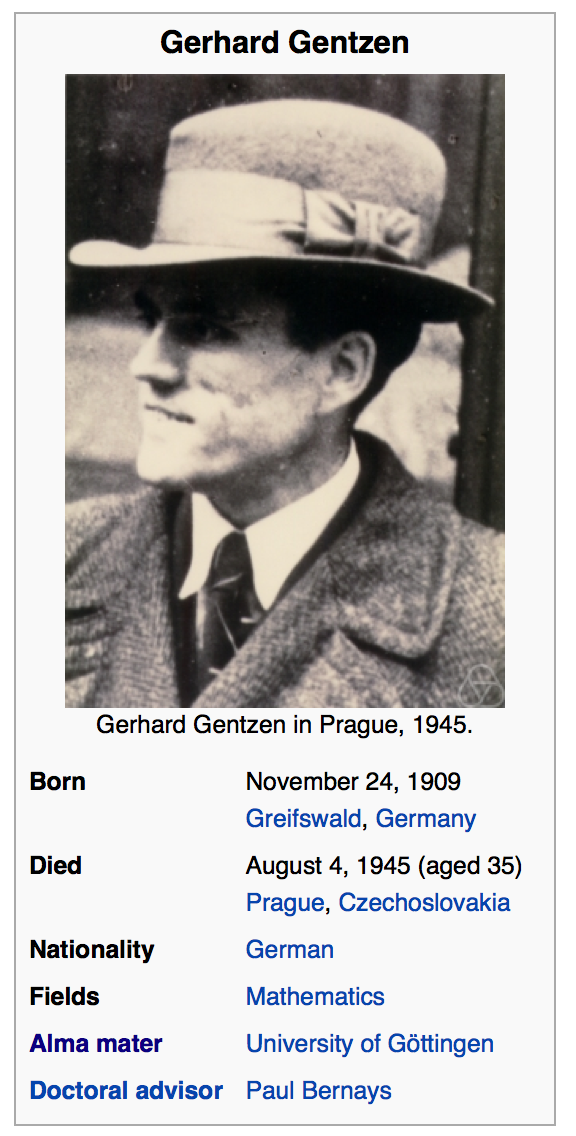
\includegraphics[height=0.8\textheight]{./gentzen-infobox.png}
  \end{figure}
\end{frame}

% Infobox hierarchy
\begin{frame}
  \frametitle{Infobox}
  Λαμβάνουμε:
  \begin{itemize}
  \item Χαρακτηριστικά από τον πίνακα του infobox
  \item Την κατηγορία της οντότητας από τον τύπο του infobox.
  \end{itemize}
\end{frame}

\begin{frame}
  \frametitle{Ιεραρχία των infoboxes}

  Προέρχεται από τη σελίδα List of infoboxes.
  πχ. \texttt{Template:Infobox officeholder} είναι υπο-κλάση του
  \texttt{Template:Infobox person} και έτσι:

  \vfill
  \begin{code}
    > (get-classes "Hillary Rodham Clinton")
    ("wikibase-term"
    "wikipedia-paragraphs"
    "wikibase-person"
    "wikipedia-officeholder"
    "wikipedia-person")
  \end{code}
\end{frame}

% Pipeline σ
\figframe{wikipediabase-pipeline}{WikipediaBase data pipeline}

\begin{frame}
  \frametitle{Resolvers}
  \begin{itemize}
  \item Infobox --- Χαρακτηριστικά απο το infobox
  \item Person --- Αν το άρθρο αναφέρεται σε άνθρωπο, το γένος του, η
    ημ. γέννησης κτλ
  \item Sections --- Αυτούσιο κείμενο του άρθρου
  \item Term --- συντεταγμένες, εικόνες, αριθμό, κύρια ονόματα,
    περίληψη άρθρου, URL και αριθμός λέξεων
  \item Error --- Ένδειξη ότι δεν βρέθηκε το χαρακτηριστικό.
  \end{itemize}
\end{frame}

\begin{frame}
  \frametitle{Classifiers}
  \begin{itemize}
  \item Term --- παντα \texttt{wikipedia-term}
  \item Infobox --- απο τον τύπο του infobox
  \item Person --- Ευρετικές για το αν το άρθρο αναφέρεται σε πρόσωπο.
  \end{itemize}
\end{frame}

% Provider/Aquirer σ
% Example dict with resolvers
% Example list with classifiers
\begin{frame}
  \frametitle{Provider/Acquirer model}

  Διαχωρισμός της λογικής που σχετίζεται με το χειρισμό δεδομένων απο
  τη λογική που καθορίζει τις πηγές της.

  \vfill

  \[
    \bigcup_{p \in providers} \{ o \, : \, o \in provided(p) \}
  \]

  ή dict πρόσβαση

  \[
    \bigcup_{p \in providers} \{ (k, v)\, : \, (k, v) \in provided(p) \}
  \]

  \vfill

\end{frame}

% Synonyms π
\begin{frame}
  \frametitle{Συνώνυμα}

  Περισσότερα από ένα σύμβολα μπορεί αν αντιστοιχούν στην ίδια
  οντότητα.

  \hfill

  Μερικά σύμβολα αντιστοιχούν σε άρθρα της wikipedia άλλα όχι σε
  οντότητες χρήσιμες στο START.

\end{frame}

\begin{frame}
  \frametitle{Παραδείγματα συνωνύμων}

  \begin{itemize}
  \item Raven (Journal) \(\equiv\) Raven
  \item Russian language/Russian alphabet \(\equiv\) Russian alphabet
    \(\equiv\) Russian language
  \item Obama \(\equiv\) Barack Obama
  \item Beatles \(\equiv\) The Beales
  \end{itemize}

\end{frame}

\begin{frame}
  \frametitle{Παραδείγματα μη αποδεκτών συνωνύμων}
  \begin{itemize}
  \item File:Venn0001.svg
  \item List of infoboxes
  \item Alexander\_Pushkin\#Legacy
  \item Abraham House \(\equiv\) A. House \(\not\equiv\) House
  \end{itemize}
\end{frame}

% Date parser χ
%% Colorful example from test
\begin{frame}
  \frametitle{Αναγνώριση χρονικών διαστημάτων}
  \begin{code}
    > I am on the {\color<4->{red}12th} bus, \\
    I will be here from \textbf<9>{
      {\color<7->{violet}{\color<4-6>{red}30th}
        of {\color<3-6>{blue}september}
        {\color<5-6>{magenta}2006}} to
      {\color<8->{violet}18.7.{\color<5-7>{magenta}2007}}} \\
    \vspace{3.0}
    \onslide<2->{\textbf<9>{({\color<7->{violet}({\color<6>{red}30},
          {\color<6>{blue}9},
          {\color<6>{magenta}2006})},
        {\color<8->{violet}(18, 7, 2007)})}}
  \end{code}
  \vfill
  \begin{itemize}
  \item<3-> {\color{blue}\texttt{tag:month, tag:fullname}}
  \item<4-> {\color{red}\texttt{tag:day, tag:numeric}}
  \item<5-> {\color{magenta}\texttt{tag:year, tag:4digit}}
  \item<6-> {\color<7->{violet}{\color<6>{red}\texttt{\{day,numeric\}}} of
      {\color<6>{blue}\texttt{\{month,fullname\}}}
      {\color<6>{magenta}\texttt{\{tag:year\}}}}
  \item<8-> \texttt{{\color{violet}\{day,number\}.\{month,number\}.\{year\}}}
  \item<9-> \textbf{{\color<9->{violet}\texttt{\{date\}}} to
      {\color<9>{violet}\texttt{\{date\}}}}
  \end{itemize}
\end{frame}

\section{Wikipedia Mirror}

\begin{frame}
  \frametitle{Τι είναι το Wikipedia Mirror}

  Ένα πρόγραμμα που παράγει κλώνους της wikipedia που τρέχουν σε ένα
  τοπικό μηχάνημα.

\end{frame}

\begin{frame}
  \frametitle{Διαδικασία}
  \begin{itemize}
  \item<2-> Στήσιμο του server stack
  \item<3-> Εγκατάσταση του Mediawiki
  \item<4-> Κατέβασμα και αποκωδικοποίηση των wikipedia dumps
  \item<5-> Φόρτωση των dumps στη wikipedia
  \item<6-> Ρύθμιση του mediawiki να μιμείται τη wikipedia
  \item<7-> {\color{gray}Ρύθμιση της βάσης δεδομένων για επιδόσεις
      συγκρίσιμες με wikipedia.org}
  \end{itemize}
\end{frame}

% Mediawiki stack σ
\begin{frame}
  \frametitle{Mediawiki Stack}

  \begin{itemize}
  \item Wikipedia configuration, \textbf<2>{database (MySQL)} etc
  \item \textbf<2>{Mediawiki}
  \item \textbf<2>{PHP}
  \item \textbf<2>{Apache}
  \item \textbf<2>{Linux}
  \end{itemize}
  \vfill
  \onslide<2>{\textbf{Bitnami!}}
  \vfill
\end{frame}

% Wikipedia dumps
\begin{frame}
  \frametitle{Περιεχόμενα βάσης δεδομένων}

  Μηνιαία snapshots ολόκληρης της βάσης (εκτός απ' τα extensions και
  τους χρήστες).
  \vfill
  \texttt{https://dumps.wikimedia.org/enwiki/latest/} \vfill
\end{frame}

% Mwdumper
\begin{frame}
  \frametitle{Mwdumper}

  Μετατροπή απο XML σε MySQL: \bf{mwdumper}
\end{frame}
% Bugs

\begin{frame}
  \frametitle{xerces bug} Stack overflow στην αποκωδικοποίηση κάποιων
  άρθρων απο την XML library (xerces).
  \vfill
  \begin{itemize}
  \item<2-> Γνωστό bug άλλα δύσκολα αναπαράξιμο.
  \item<3-> Μονό του το προβληματικό άρθρο δεν έσπαγε.
  \item<4-> Καλυμμένο με κενά έσπαγε.
  \item<5-> Αφαιρετέο από το XML αρχείο δούλευε.\onslide<6>
    Αυτοματοποιήσουμε αυτή τη διαδικασία.
  \end{itemize}
\end{frame}

% Performance

\begin{frame}
  \frametitle{Επιδόσεις}
  \begin{itemize}
  \item \textbf{CPU:} Xeon E5-1607 3GHz 4-Core 64 bit
  \item \textbf{Main memory:} 64G
  \item \textbf{HDD:} (spinning disk) 500GB + 2Tb
  \end{itemize}
\end{frame}

\begin{frame}
  Επιδόσεις δημιουργίας της βάσης (ανάλογα τη φορά):

  \begin{itemize}
  \item Προεπεξεργασία των dumps ~10 λεπτά
  \item Δημιουργία της βάσης ~10 ώρες
  \end{itemize}
\end{frame}

\begin{frame}
  \frametitle{Runtime Επιδόσεις}

  Απαγορευτικές για την ομαλή λειτουργία του START. Για το άρθρο του
  Barack Obama:
  \begin{itemize}
  \item Χωρίς βελτιστοποιήσεις ~10s κατ ευθείαν στη βάση
  \item Με κάποιες βελτιστοποιήσεις ~7s κατ ευθείαν στη βάση
  \end{itemize}
\end{frame}

\begin{frame}
  \frametitle{Ρυθμίσεις MySQL}

  Βελτιστοποιήσεις στη βάση που επιχειρήθηκαν:

  \begin{itemize}
  \item \texttt{innodb\_buffer\_pool\_size} \(\in\) (16Μ, 5GB)
  \item Απενεργοποίηση της \texttt{fsync}
  \item \texttt{innodb\_io\_capacity} ήταν μεγαλύτερη από το bandwidth
    του δίσκου.
  \item \texttt{SET AUTOCOMMIT = 0; SET FOREIGN\_KEY\_CHECKS=0;} κατά τη
    διάρκεια των dumps.
  \end{itemize}
\end{frame}

\section{Επίλογος}

\begin{frame}
  \frametitle{Ευχαριστίες}

  Ευχαριστώ τους καθηγητές μου κ Σγάρμπα, κ Katz και κ Φακωτάκη.

\end{frame}

\begin{frame}
  \frametitle{Mandatory Dijkstra quote}

  \vfill
  \textit{The question of whether Machines Can Think... is about as relevant as the question of whether Submarines Can Swim.\\
  \hfill --- Edsger W. Dijkstra}
  \vfill

\end{frame}

\begin{frame}
  \frametitle{Links}
  \begin{itemize}
  \item \texttt{https://github.com/infolab-csail/WikipediaBase}
  \item \texttt{https://github.com/infolab-csail/wikipedia-mirror}
  \item \texttt{https://github.com/fakedrake/overlay\_parse}
  \item \texttt{https://bitnami.com/}
  \item \texttt{https://en.wikipedia.org/}
  \item \texttt{https://dev.mysql.com/doc/refman/5.5/en/innodb-parameters.html}
  \end{itemize}
\end{frame}
\end{document}
